\section{Methodological Approach}\label{sec:methodological_approach}
The methodological approach in this study is described in the subsection below and visualized in \cref{fig:methodological_approach}. 

\subsection{Data Collection}\label{sec:data_collection}
The datasets used to conduct this study are all based on three public sources: a) Voyage Reports b) \ac{cmems} and c) \ac{era5}. 

\subsubsection{Voyage Reports}\label{sec:voyage_reports}
Voyage reports data, sometimes also referred to as noon reports, are data that are captured manually and reported by the chief engineer daily at noon, hence the name, and then sent by the ship master to the shipping company and shore management to report operational and performance status of the vessel as mentioned by Ran et al.~\citep{YAN2021102489}. These reports are mandated by \ac{imo} to meet regulatory requirements such as \ac{dcs}, which mandate since 2019, all ships over 5,000 gross tons to report their daily aggregated fuel consumption as mentioned by \ac{imo}~\citep{imoIMODataCollection2023}. 

Noon reports contain navigational information (e.g., latitude and longitude), operational information (e.g., speed over ground, engine rpm), and weather information (e.g., wind speed and swell force). A raw sample of the reports used in the study is shown in \cref{tab:voyage_report_raw_samples_subset} and for a full list of the parameters retrieved together with their unit of measurements see \ref{tab:voyages_raw_parameters} in appendix. 

\clearpage
\begin{table}[h!]
       \centering
       \caption{Voyage Report Raw Samples Subset}
       \resizebox{\textwidth}{!}{%
       \begin{tabular}{lll}
       \toprule
       {} &             \textbf{position} & \textbf{current\_speed\_over\_ground} \\
       \textbf{date}                &                      &                           \\
       \midrule
       16 NOV 2021 1200LT  &  02-16.0N\textbackslash n101-52.5E &                      13.6 \\
       17 NOV 2021 1200LT  &  05-57.0N\textbackslash n097-39.5E &                      13.5 \\
       18 NOV 2021 1200LT  &  06-15.4N\textbackslash n092-16.2E &                      13.7 \\
       19 Nov 2021\textbackslash n1200LT &  05-47.4N\textbackslash n086-37.4E &                      13.5 \\
       \bottomrule
       \end{tabular}%
       }
       \label{tab:voyage_report_raw_samples_subset}
\end{table}

The reports originated from a bulk carrier vessel named Hercules, shown in \cref{fig:hercules}. 
For an overview of the vessel particulars and power specifications, see \cref{tab:hercules_particulars,tab:hercules_power_specifications}. 

\begin{table}[h!]
    \centering
    \caption[Hercules Particulars]{Hercules Particulars. Source ~\citep{marinetraffic}}
    \label{tab:hercules_particulars}
    \begin{tabular}{ll}
    \hline
    IMO                    & 9642382      \\
    MMSI                   & 636015986    \\
    General Type           & Cargo        \\
    Specific Type          & Bulk Carrier \\
    Gross Tonnage          & 41,104       \\
    Summer Deadweight (t)  & 75,200       \\
    Length overall LOA (m) & 225          \\
    Width (m)              & 32.26        \\
    Beam (m)               & 32           \\
    Year Built             & 2013        
    \end{tabular}
\end{table}

The timespan of data used is from 16 November 2021 to 21 November 2022 in daily frequency, which amounts to 296 samples and 28 parameters. 

Since voyage reports are logged manually, specific measurements generally will have human errors, specifically for weather and sea parts of the measurements recorded since they are gauged. Moreover, the weather parameters logged in these reports are limited to a handful of parameters and also missing many signals. This motivated the inspection of other more reliable and quality weather and sea state data that could be fused to produce better models. 

Our investigation revealed that the highest quality data vendors that fulfill this are using \ac{cmems} as well as the \ac{era5}, which is, according to Li et al.~\citep{liDataFusionMachine2022}, what windy~\citep{windy} uses internally, which is an application that is widely adopted for assessing maritime navigation in real-time by providing reliable weather forecasts in the open ocean.

\begin{figure}
    \centering
    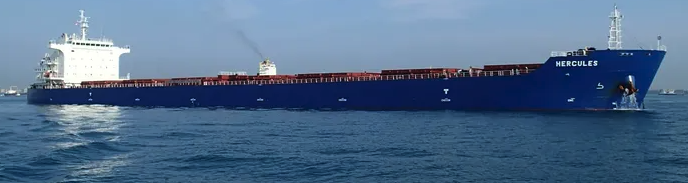
\includegraphics[width=1\linewidth]{hercules}
    \caption{Hercules Vessel}
    \label{fig:hercules}
\end{figure}

\begin{table}[h!]
    \centering
    \caption{Hercules Power Specifications}
    \label{tab:hercules_power_specifications}
    \begin{tabular}{ll}
    \hline
    Engine Type       & Diesel      \\
    Engine Builder    & MAN B\&W    \\
    Model             & 5S60MC-C    \\
    RPM               & 105         \\
    Stroke Type       & 2           \\
    Cylinder Stroke   & 2400        \\
    Cylinder Bore     & 600         \\
    Total Power (kw)  & 8833        \\
    Propulsion type   & Fixed Pitch \\
    Propulsion number & 1           \\
    Speed             & 14.5       
    \end{tabular}
    \end{table}

        


\subsubsection{\ac{cmems}}\label{sec:cmems}

\ac{cmems} provides high-quality data on the ocean, which includes information on the state of the Blue (physical), White (sea ice), and Green (biogeochemical) ocean on a global and regional scale. It integrates satellite observations, in-situ measurements, and advanced numerical models. It offers information specifically on the ocean, such as currents, sea level, salinity, and biogeochemical parameters ~\citep{copernicusmarineservice}.

It has a whole host of different products, and the product selected for this study is Global Ocean Physics Analysis and Forecast~\citep{cmems2024global}, which was inspired by the study Li et al.~\citep{liDataFusionMachine2022}.

The product comprises five different datasets, each with different parameters. \cref{tab:cmems_data_description,tab:cmems_raw_samples} describe the metadata and a sample of the raw data used. For details on the parameters together with their unit of measurements see \cref{tab:cmems_raw_parameters} in appendix. 

Since \ac{cmems} focuses on oceanic data, another data source was needed to be fused, which is \ac{era5}, which completes environmental data by covering atmospheric reanalysis that includes information on the climate such as wind speed, wind direction, and temperatures. 

\begin{table}[!ht]
    \centering
    \caption{Global Ocean Physics Analysis and Forecast Data Description}
    \resizebox{\textwidth}{!}{%
    \begin{tabular}{ll}
    \hline
        \textbf{Dataset ID} & \textbf{Short Description} \\ \hline
        cmems\_mod\_glo\_phy\_anfc\_0.083deg\_P1D-m & 2D daily mean of various different measurements \\ 
        cmems\_mod\_glo\_phy-cur\_anfc\_0.083deg\_P1D-m & 3D daily mean horizontal currents information from top to bottom \\ 
        cmems\_mod\_glo\_phy-thetao\_anfc\_0.083deg\_P1D-m & 3D daily mean potential temperature information from top to bottom \\ 
        cmems\_mod\_glo\_phy-so\_anfc\_0.083deg\_P1D-m & 3D daily mean salinity information from top to bottom \\ 
        cmems\_mod\_glo\_phy-wcur\_anfc\_0.083deg\_P1D-m & 3D daily mean vertical current information from top to bottom \\ \hline
    \end{tabular}%
    }
    \label{tab:cmems_data_description}
\end{table}

\begin{table}[!ht]
    \centering
    \caption{Global Ocean Physics Analysis and Forecast Raw Samples}
    \resizebox{\textwidth}{!}{%
    \begin{tabular}{llllrrrrr}
        \toprule
                &       &            &            &  \textbf{ist} &     \textbf{mlotst} &          \textbf{pbo} &  \textbf{siage} &  \textbf{sialb} \\
                \textbf{depth} & \textbf{latitude} & \textbf{longitude} & \textbf{time} &      &            &              &        &        \\
        \midrule
        0.494025 & -36.0 & -43.000000 & 2021-11-16 &  0.0 &  20.942480 &  5003.330078 &    0.0 &  0.066 \\
                &       & -42.916656 & 2021-11-16 &  0.0 &  20.706240 &  5009.921875 &    0.0 &  0.066 \\
                &       & -42.833328 & 2021-11-16 &  0.0 &  20.484440 &  5001.324219 &    0.0 &  0.066 \\
                &       & -42.750000 & 2021-11-16 &  0.0 &  19.690535 &  5000.277344 &    0.0 &  0.066 \\
                &       & -42.666656 & 2021-11-16 &  0.0 &  19.470037 &  5000.562988 &    0.0 &  0.066 \\
        \bottomrule
        \end{tabular}%
    }
    \label{tab:cmems_raw_samples}
\end{table}


\subsubsection{\ac{era5}}\label{sec:era5}

\ac{era5} is a global atmospheric reanalysis dataset produced by \ac{ecmwf}. It provides hourly data on the climate from 1959 to the present, combining model data with observations Hersbach et al.~\citep{hersbach2023era5}.

The data obtained were selected from the product, hourly data on single levels from 1940 to the present, which was inspired by the study ~\citep{liDataFusionMachine2022}. This provided 61 parameters related to the climate that were used to test if they contributed to improving the overall performance.

A short description of the dataset used together with a sample on the raw measurements are depicted in~\cref{tab:era5_data_description,tab:era5_raw_samples}.
For details on the used parameters their unit of measurements see \cref{tab:era5_raw_parameters} in appendix.

\clearpage

\begin{table*}[!ht]
    \centering
    \caption{ERA5 Hourly on Single Levels Data Description}
    \resizebox{\textwidth}{!}{%
    \begin{tabular}{ll}
    \hline
        Data type & Gridded \\
        Projection & Regular latitude-longitude grid \\ 
        Horizontal coverage & Global \\ 
        Horizontal resolution & Reanalysis: 0.25° x 0.25° (atmosphere), 0.5° x 0.5° (ocean waves).  \\ 
        Temporal coverage & 1940 to present \\ 
        Temporal resolution & Hourly \\ 
        File format & GRIB \\ 
        Update frequency & Daily \\ \hline
    \end{tabular}%
    }
    \label{tab:era5_hourly_on_single_levels_data_description}
\end{table*}

\begin{table}[!ht]
        \centering
        \caption{ERA5 Hourly on Single Levels Raw Samples}
        \resizebox{\textwidth}{!}{%
        \begin{tabular}{lllrrrrr}
        \toprule
                &       &            &  \textbf{number} &   \textbf{step} &  \textbf{surface} &      \textbf{u100} &       \textbf{v100} \\
                \textbf{latitude} & \textbf{longitude} & \textbf{time} &         &        &          &           &            \\
        \midrule
        56.0 & -43.0 & 2021-11-01 &       0 & 0 days &      0.0 &  4.457072 &   3.199743 \\
                &       & 2021-11-02 &       0 & 0 days &      0.0 &  4.228130 &  12.664192 \\
                &       & 2021-11-03 &       0 & 0 days &      0.0 &  6.418368 &   6.450352 \\
                &       & 2021-11-04 &       0 & 0 days &      0.0 &  4.549166 &   0.413618 \\
                &       & 2021-11-05 &       0 & 0 days &      0.0 &  3.050886 &  -1.523218 \\
        \bottomrule
        \end{tabular}%
        }
        \label{tab:era5_raw_samples}
\end{table}

Data preprocessing significantly contributes to the generalization performance of a supervised \ac{ml} algorithm~\citep{xieFuelConsumptionPrediction2023}, and therefore, this was carried out next. 


\subsection{Data Preprocessing and Fusing}\label{sec:data_preprocessing_and_fusing}

To achieve the best results, it is also crucial to carefully balance the need to clean the data with maintaining the integrity of the raw data. Hence, having a consistent pipeline was crucial to avoid data leakage during training and ensure reproducibility. Therefore, Sklearn pipelines have been used, which are sequential lists of steps that could be applied to the data. Each step could be a transformation or an estimator. This standardized the process of building models, which ensures consistency and reproducibility.

At first, the data were converted from Excel to pandas data frames so that the tools could be applied to them. Then, some columns were renamed to have more meaningful names. Then, any observation involving a shift in state in any of the following (Loading Operation, Anchor, Bunkering Operation, Discharging Operation, VSL Anchored, and Drifting) was removed from the data since it had empty values across all measurements. Next, some alignments were done to map the noon reports to the environmental sources. These alignments included that the dates have been converted from Geneva to \ac{utc}. The geographical positions have been converted from \ac{ddm} to \ac{dd}.
Then, some measurements have been derived from the raw measurements. This includes expanding the draft to a forward draft and an aft draft. Then, the trim from the draft values is computed. Then, the date parameters were expanded into year, month, day, and season based on whether the ship's location was in the north or south hemisphere. Then, the main engine's fuel was derived by adding two different fuel types, mainly ultra-low sulfur fuel and gas fuel. Ultimately, this rolled up to total fuel, which is based on adding fuel used in the main engine, the boilers, and any auxiliary systems. Lastly, the voyage segments were derived, which is the clustering of different port-to-port trips made by the vessel.
Some types of conversions were necessary to accommodate machine learning. This involved transforming some columns, such as total fuel or propeller slip, to floats while converting other measurements to integers or objects.
Next, \ac{cmems} and \ac{era5} data were fused to the voyage data. Since \ac{era5} data are in high resolution hourly, it was averaged to daily noons, reducing the overall size of the data from 0.5 TB to 10GB. The fusing is then done by extracting climate and ocean parameters and matching them with the voyage time and geographical location.
Lastly, linear interpolation with backward fill was carried out to fill for missing observations where climate and ocean measurements along ship voyages were missing. Linear interpolation fills missing values based on the mean of the upper and lower values. Then, the removal of observations and the dropping of some measurements were necessary. This involved the removal of columns that add no value to the predictive power, such as constant parameters or parameters with lots of missing values greater than 5\%, which only added noise. Examples include current speed over the ground since it is correlated with an average speed over the ground or next port, etc. The outliers in the response variable were identified in roughly 3-5 observations and eliminated, and this proved to improve the overall predictive power, as discussed in \cref{sec:results}. Finally, based on the observation made on fuel consumption relation with speed, which is discussed in \cref{sec:results}, the start-up acceleration instances where the speed is high but fuel consumption is lower than usual for bulk carrier of this size have been identified which aligns with Xie et al.~\citep{xieFuelConsumptionPrediction2023} and a threshold was set to 15 ton/day as a minimum where selected based on a typical bulk carrier of this particulars \cref{tab:hercules_particulars}.
The final data used after preprocessing for training were 266-noon reports and 94 parameters, including the response variable. The historical visited waypoints by the vessel is shwon in \cref{fig:waypoints_visited_frequency}. 
It illustrates the spatial distribution of the case study vessel's operational frequency across global maritime routes. Areas of higher intensity (red and orange regions) indicate zones with more frequent vessel presence, while cooler colors (green to blue) represent lower visitation frequencies. The heatmap clearly reveals the vessel’s primary operational corridors, which align with major global shipping lanes, including:  

\begin{itemize}
    \item The Strait of Malacca and South China Sea, indicating intensive activity in Southeast Asian waters
    \item The Bay of Bengal and Arabian Sea, with a prominent route extending through the Suez Canal into the Mediterranean Sea
    \item Southern passages around Africa (Cape of Good Hope) and connectivity to the South Atlantic
    \item Eastward trajectories suggest routes to Australia and the Western Pacific.

\end{itemize}

This spatial footprint highlights the vessels integration in key international trade routes and underscores the relevance of the selected case study vessel for analyzing fuel consumption and voyage dynamics in real-world global maritime operations.
A sample code from the source code used for the data transformation Source Code \ref{src:preprocessing_pipeline} demonstrate the applied transformational steps in the pipeline.

\begin{figure}
    \centering
    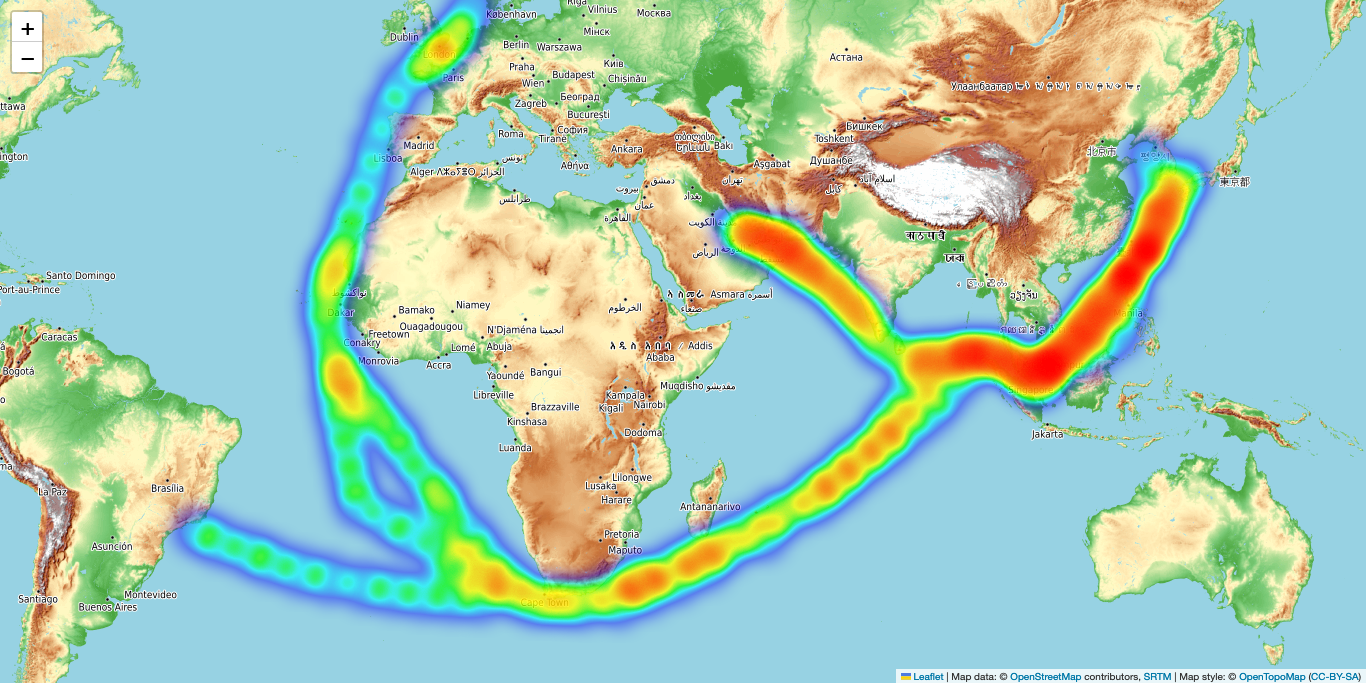
\includegraphics[width=1\linewidth]{waypoints_visited_frequency}
    \caption{Waypoints Visited}
    \label{fig:waypoints_visited_frequency}
\end{figure}


\begin{figure}
    \lstinputlisting[
        language=Python,
        firstline=56,
        lastline=76,
        caption={Preprocessing Pipeline},
        label={src:preprocessing_pipeline}
    ]{preprocessing_pipeline.py}
\end{figure}

\clearpage

\subsection{Models Development}\label{sec:models_development}

The model development procedure were divided into three parts: a) Baseline Model, b) Feature Analysis and c) Advanced Model. 

\subsection{Baseline Model}\label{sec:baseline_model}

The baseline model assesses overall performance using only one main predictor which is: Engine \ac{rpm}, one of the most essential variables in predicting ship \ac{fc}. 
This is more relevant than using \ac{sog} as discussed in \cref{sec:results} and also in alinment with the findings by ~\citep{Uyanik2022}.

This predictor was used to produce a baseline model without taking into consideration any environmental parameters nor operational factors in order to assess the extend 
to which variations in the \ac{fc} could be explained. For that multiple estimators with default settings from various categories such as: Linear, Tree Based, Support Vector Regression and Ensembles have been deployed. 
The estimators considered are shown in Source Code \ref{src:ml_estimators}.  

\clearpage

\begin{figure}
    \lstinputlisting[
        language=Python,
        firstline=17,
        lastline=30,
        caption={ML Estimators},
        label={src:ml_estimators}
    ]{evaluate_models.py}
\end{figure}

\subsubsection{\ac{rr}}\label{sec:rr}

\ac{rr} is a type of linear regression models also referred to as Tikhonov Regularization and developed by Hoerl et al.~\citep{hoerl1970ridge}
which is an addition of the widely known \ac{ols} regression where it introduces penalization propotional to the square of the coefficient to address any 
multicollinearity and overfitting cases. The mathemtical formulation for the cost function is depicted in \cref{eq:ridge_cost}.  

\begin{equation}
    \min_{\beta} \| y - X\beta \|_2^2 + \lambda \|\beta\|_2^2
\label{eq:ridge_cost}
\end{equation}
    
Where:
\begin{itemize}
    \item \( \| y - X\beta \|_2^2 = \sum_{i=1}^n (y_i - X_i \beta)^2 \): Residual sum of squares.
    \item \( \|\beta\|_2^2 = \sum_{j=1}^p \beta_j^2 \): L2 regularization term.
    \item \( \lambda \): Regularization parameter controlling the trade-off between minimizing the residual sum of squares and shrinking the coefficients.
\end{itemize}

\subsubsection{\ac{rf}}\label{sec:rf}

\ac{rf} is an ensemble learning method. It is an enhancement to \ac{dt} which originated by Breiman et al.~\citep{breiman2001random}. 
It is an ensemble in the sense that it combines multiple \ac{dt} to improve accuracy and reduce overfitting. 
It operates by constructing multiple trees and then outputing the mean prediction for regression tasks. 
The mathemtical formulation of the cost function is depicted in \cref{eq:rf_cost}. 

\begin{equation}
    \mathcal{L} = \frac{1}{N} \sum_{i=1}^{N} \left( y_i - \frac{1}{T} \sum_{t=1}^{T} \hat{y}_{i,t} \right)^2
    \label{eq:rf_cost}
    \end{equation}
    
Where:
\begin{itemize}
    \item \( N \): Number of samples.
    \item \( T \): Number of trees in the forest.
    \item \( y_i \): Actual value of the \( i \)-th sample.
    \item \( \hat{y}_{i,t} \): Prediction for the \( i \)-th sample by the \( t \)-th tree.
    \item \( \frac{1}{T} \sum_{t=1}^{T} \hat{y}_{i,t} \): Average prediction across all trees.
\end{itemize}

\subsubsection{\ac{svr}}\label{sec:svr}
\ac{svr} originally developed by Harris et al.~\citep{drucker1997svr}. The working principle is the transformation of data into higher-dimentional space using a kernel 
and then finding a hyperplane that best maximize marginn between different classes then the margin of tolerance is searched. 
The mathemtical formulation for the cost function is depicted in \cref{eq:svr_cost}.

\begin{equation}
\min_{\mathbf{w}, b, \xi^+, \xi^-} \frac{1}{2} \|\mathbf{w}\|^2 + C \sum_{i=1}^n (\xi_i^+ + \xi_i^-)
\label{eq:svr_cost}
\end{equation}

Subject to the following constraints:
\begin{equation}
\begin{aligned}
y_i - (\mathbf{w} \cdot \mathbf{x}_i + b) &\leq \epsilon + \xi_i^+, \quad i = 1, \dots, n, \\
(\mathbf{w} \cdot \mathbf{x}_i + b) - y_i &\leq \epsilon + \xi_i^-, \quad i = 1, \dots, n, \\
\xi_i^+, \, \xi_i^- &\geq 0, \quad i = 1, \dots, n.
\end{aligned}
\label{eq:svr_constraints}
\end{equation}

\begin{itemize}
    \item \( \mathbf{w} \): The weight vector defining the regression hyperplane.
    \item \( b \): The bias term in the hyperplane equation \( f(\mathbf{x}) = \mathbf{w} \cdot \mathbf{x} + b \).
    \item \( \epsilon \): The \emph{insensitivity margin} parameter, which defines a tolerance zone (or \(\epsilon\)-tube) around the hyperplane where deviations are not penalized.
    \item \( \xi_i^+ \): Slack variable representing the amount by which a predicted value exceeds the upper bound of the \(\epsilon\)-tube.
    \item \( \xi_i^- \): Slack variable representing the amount by which a predicted value falls below the lower bound of the \(\epsilon\)-tube.
    \item \( C \): Regularization parameter that controls the trade-off between the model's complexity (\( \frac{1}{2} \|\mathbf{w}\|^2 \)) and the penalty for deviations outside the \(\epsilon\)-tube (\( \sum_{i=1}^n (\xi_i^+ + \xi_i^-) \)).
    \item \( y_i \): The true target value for the \(i\)-th data point.
    \item \( \mathbf{x}_i \): The feature vector for the \(i\)-th data point.
    \item \( n \): The total number of data points in the training set.
\end{itemize}

\subsubsection{\ac{xgboost}}\label{sec:xgboost}

\ac{xgboost} is a type of both ensemble and gradient boosting developed by Tianqi et al.~\citep{chen2016xgboost}. Its main working principle relies on building multiple \ac{dt} similar to 
\ac{rf} but it differs that its based on boosting where trees are trained sequentially to correct the errors of its predecessor unlike \ac{rf} which is based on bagging i.e bootstap aggregation. 
The mathemtical formulation for its cost function is depicted in \cref{eq:xgboost_cost}.

\begin{equation}
\mathcal{L}(t) = \sum_{i=1}^n \ell(y_i, \hat{y}_i^{(t)}) + \sum_{k=1}^t \Omega(f_k),
\label{eq:xgboost_cost}
\end{equation}

where:
\begin{itemize}
    \item \( \ell(y_i, \hat{y}_i^{(t)}) \): Loss function for the \(i\)-th data point (e.g., Mean Squared Error or Mean Absolute Error).
    \item \( \Omega(f_k) = \gamma T + \frac{1}{2} \lambda \|\mathbf{w}\|^2 \): Regularization term for the \(k\)-th tree, where:
    \begin{itemize}
        \item \( T \): Number of leaves in the tree.
        \item \( \gamma \): Regularization parameter for leaf nodes.
        \item \( \lambda \): L2 regularization parameter for leaf weights.
        \item \( \mathbf{w} \): Vector of leaf weights.
    \end{itemize}
    \item \( t \): Current boosting iteration.
    \item \( n \): Number of data points.
\end{itemize}

\subsubsection{Validation of the methods}\label{sec:validation_of_the_methods}

The estimators have been evaluated using cross-validation technique more specifically using 5-fold cross validation. 
The basic principle behind this technique is that data split randomly into k subsets/folds and then the model is trainined in k-1 while getting tested in remaining folds till k times is reached.
This make sure that no overfitting or underfitting phenomenas occur when reporting the final error metrics as its also reported as an average across all folds. 

The technique became prominant in \ac{ml} space for validating models by Stone~\citep{stone1974cross} and its mathemtical formulation is shown below:

Let the dataset \( D \) consist of \( n \) data points, and we split it into \( k \) subsets or folds: 
\begin{equation}
    D = \{D_1, D_2, \dots, D_k\}
\end{equation}
where \( D_i \) is the \( i \)-th fold. 

For each fold \( i \), we train the model on the data from all folds except the \( i \)-th fold, and test it on the \( i \)-th fold. That is, the training data is 
\begin{equation}
    D_{\text{train}} = D \setminus D_i, \quad \text{and the test data is } D_{\text{test}} = D_i.
\end{equation}

The error for fold \( i \) is given by:
\begin{equation}
    \mathcal{E}_i = \frac{1}{|D_i|} \sum_{x_j \in D_i} \mathcal{L}(f(x_j), y_j)
\end{equation}
where:
\begin{itemize}
    \item \( \mathcal{L} \) is the loss function (e.g., Mean Squared Error for regression)
    \item \( f(x_j) \) is the predicted value for the data point \( x_j \)
    \item \( y_j \) is the true value for \( x_j \).
\end{itemize}

The overall cross-validation error is the average error across all \( k \) folds:
\begin{equation}
    \mathcal{E}_{\text{CV}} = \frac{1}{k} \sum_{i=1}^{k} \mathcal{E}_i.
\end{equation}
\clearpage
The models are evaluated using the following performance and error metrics: 
\begin{itemize}
    \item \ac{r2}
    \item Adjusted \ac{r2}
    \item \ac{rmse} 
    \item \ac{mae}
\end{itemize}

\subsubsection{R2 and Adjusted R2}\label{sec:r2_and_adjusted_r2}
\ac{r2} also known as coefficient of determination developed by Francis~\citep{galton1886regression} and it represents the variance in the dependent variable 
that is explained by the independent variables. The adjusted \ac{r2} is a modified version of \ac{r2} developed by George~\citep{mcnemar1978statistical}. Its similar to 
\ac{r2} with slight difference that it take into account the number of predictors in the model so that 
adding more independent variables dont purely inflate \ac{r2}. It works by penalizing the model for adding more independent variables 
that dont contribute with additional information. 

The mathematical formulation for both performance metrics are shown in \cref{eq:r2,eq:r2_adj}.

\begin{equation}
    R^2 = 1 - \frac{\sum_{i=1}^{n} (y_i - \hat{y}_i)^2}{\sum_{i=1}^{n} (y_i - \bar{y})^2}
\label{eq:r2}
\end{equation}

where:
\begin{itemize}
    \item \(y_i\) is the actual value of the \(i\)-th observation.
    \item \(\hat{y}_i\) is the predicted value for the \(i\)-th observation
    \item \(\bar{y}\) is the mean of the actual values.
    \item \(n\) is the number of data points.
\end{itemize}
\clearpage
The formula for Adjusted \(R^2\) is given by:

\begin{equation}
    \bar{R}^2 = 1 - \left(1 - R^2\right) \frac{n-1}{n-p-1}
\label{eq:r2_adj}
\end{equation}

where:
\begin{itemize}
    \item \(n\) is the number of observations.
    \item \(p\) is the number of predictors in the model.
\end{itemize}

\subsubsection{RMSE and MAE}\label{sec:rmse_and_mae}
\ac{rmse} measures the average magnitude of the errors between the predicted and observed values. 
Its first popularized by Willmott et al.~\citep{willmott1985rmse} and it gives an idea of how concentrated the 
data is around the line of best fit. The mathematical formulation for both error metrics are shown in \cref{eq:rmse,eq:mae}.

\begin{equation}
    \text{RMSE} = \sqrt{\frac{1}{n} \sum_{i=1}^{n} (y_i - \hat{y}_i)^2}
    \label{eq:rmse}
\end{equation}

where:
\begin{itemize}
    \item \(y_i\) is the actual value of the \(i\)-th observation,
    \item \(\hat{y}_i\) is the predicted value for the \(i\)-th observation,
    \item \(n\) is the total number of data points.
\end{itemize}

\ac{mae} is a widely used error metric that concentrate on measuring the average of absolute
errors. Huber et al.~\citep{huber1964robust} was the first to put the groundwork for error metrics based on absolute deviations. 
Its less sensitive to extreme values as compared to \ac{rmse} where it average squared errors by squaring the differences and it gives more weight to larger errors. 

\begin{equation}
    \text{MAE} = \frac{1}{n} \sum_{i=1}^{n} |y_i - \hat{y}_i|, \quad 
    \label{eq:mae}
\end{equation}

where:
\begin{itemize}
    \item $n$ is the total number of data points,
    \item $y_i$ is the actual value of the $i$-th data point,
    \item $\hat{y}_i$ is the predicted value for the $i$-th data point,
    \item $|y_i - \hat{y}_i|$ is the absolute error for the $i$-th data point.
\end{itemize}

\subsection{Features Analysis}\label{sec:feature_analysis}

Next, more features needed to be exaimined in order to evaluate its relevance for predicting \ac{fc}. \ac{rf} have been used to evaluate and quantify feature importance. 
Random Forest calculates feature importance by evaluating how much each feature contributes to reducing the impurity 
using Gini impurity in the decision trees. For each feature, measure the total decrease in Gini impurity that results from splitting on this feature, 
averaged over all trees. For mathematical formulation see \cref{eq:feature_importance}. 

\begin{equation}
    \text{Importance of feature } j = \sum_{t=1}^{T} \frac{N_t}{N} \cdot \left( \text{Impurity before split}_t - \text{Impurity after split}_t \right)
    \label{eq:feature_importance}
\end{equation}

\begin{itemize}
    \item $T$ is the total number of trees in the Random Forest.
    \item $N_t$ is the number of samples in tree $t$.
    \item $N$ is the total number of samples in the dataset.
    \item $\text{Impurity before split}_t$ is the impurity of node before splitting (e.g., Gini impurity for classification).
    \item $\text{Impurity after split}_t$ is the impurity of node after splitting (again, Gini impurity or other impurity measure).
    \item The product $\frac{N_t}{N}$ weights the impurity change by the proportion of samples in each tree.
\end{itemize}

Statistical analysis reveals that the existing MLMs may be sensitive to the varying numbers of influencing factors (inputs), apparently ranging from 7 to 75 Chen et al.~\citep{chenetal2023}
A handful of the inputs variables have been identified to contribute to model accuracy as discussed in \cref{sec:results}. Next those identified features have been used to build advanced models that are then compared against baseline. 

\subsection{Advanced Model}\label{sec:advanced_model}
An advanced multivariate model was developed and compared against a baseline model in which all the selected predictors were utilized. This has revealed a tangible improvement in overall performance which is discussed in \cref{sec:results}

Then grid search was deployed to search best parameters to be used for the final model. 
Grid search is a technique that is evolved from optimization domain and made popularized by Pedregosa et al.~\citep{pedregosa2011scikit}. The general idea is that it tries to search through manually specified subsets of hyperparameter space 
to find an optimal combination that gives the best model performance. For the mathematical formulation see \cref{eq:grid_search}

\begin{equation}
    \Theta^* = \arg\max_{\Theta \in G} J\big(f(\Theta), D_{\text{val}}\big)
    \label{eq:grid_search}
    \end{equation}
    
    where:
    
    \begin{itemize}
        \item \( \Theta \): Set of hyperparameters (e.g., learning rate, regularization term).
        \item \( G \): Grid of possible hyperparameter combinations.
        \item \( J \): Objective function, such as validation accuracy or error.
        \item \( f(\Theta) \): Model parameterized by the hyperparameters \( \Theta \).
        \item \( D_{\text{val}} \): Validation dataset used to evaluate the model's performance.
        \item \( \Theta^* \): Optimal hyperparameters that maximize or minimize \( J \).
    \end{itemize}

\begin{figure}[!ht]
    \centering
    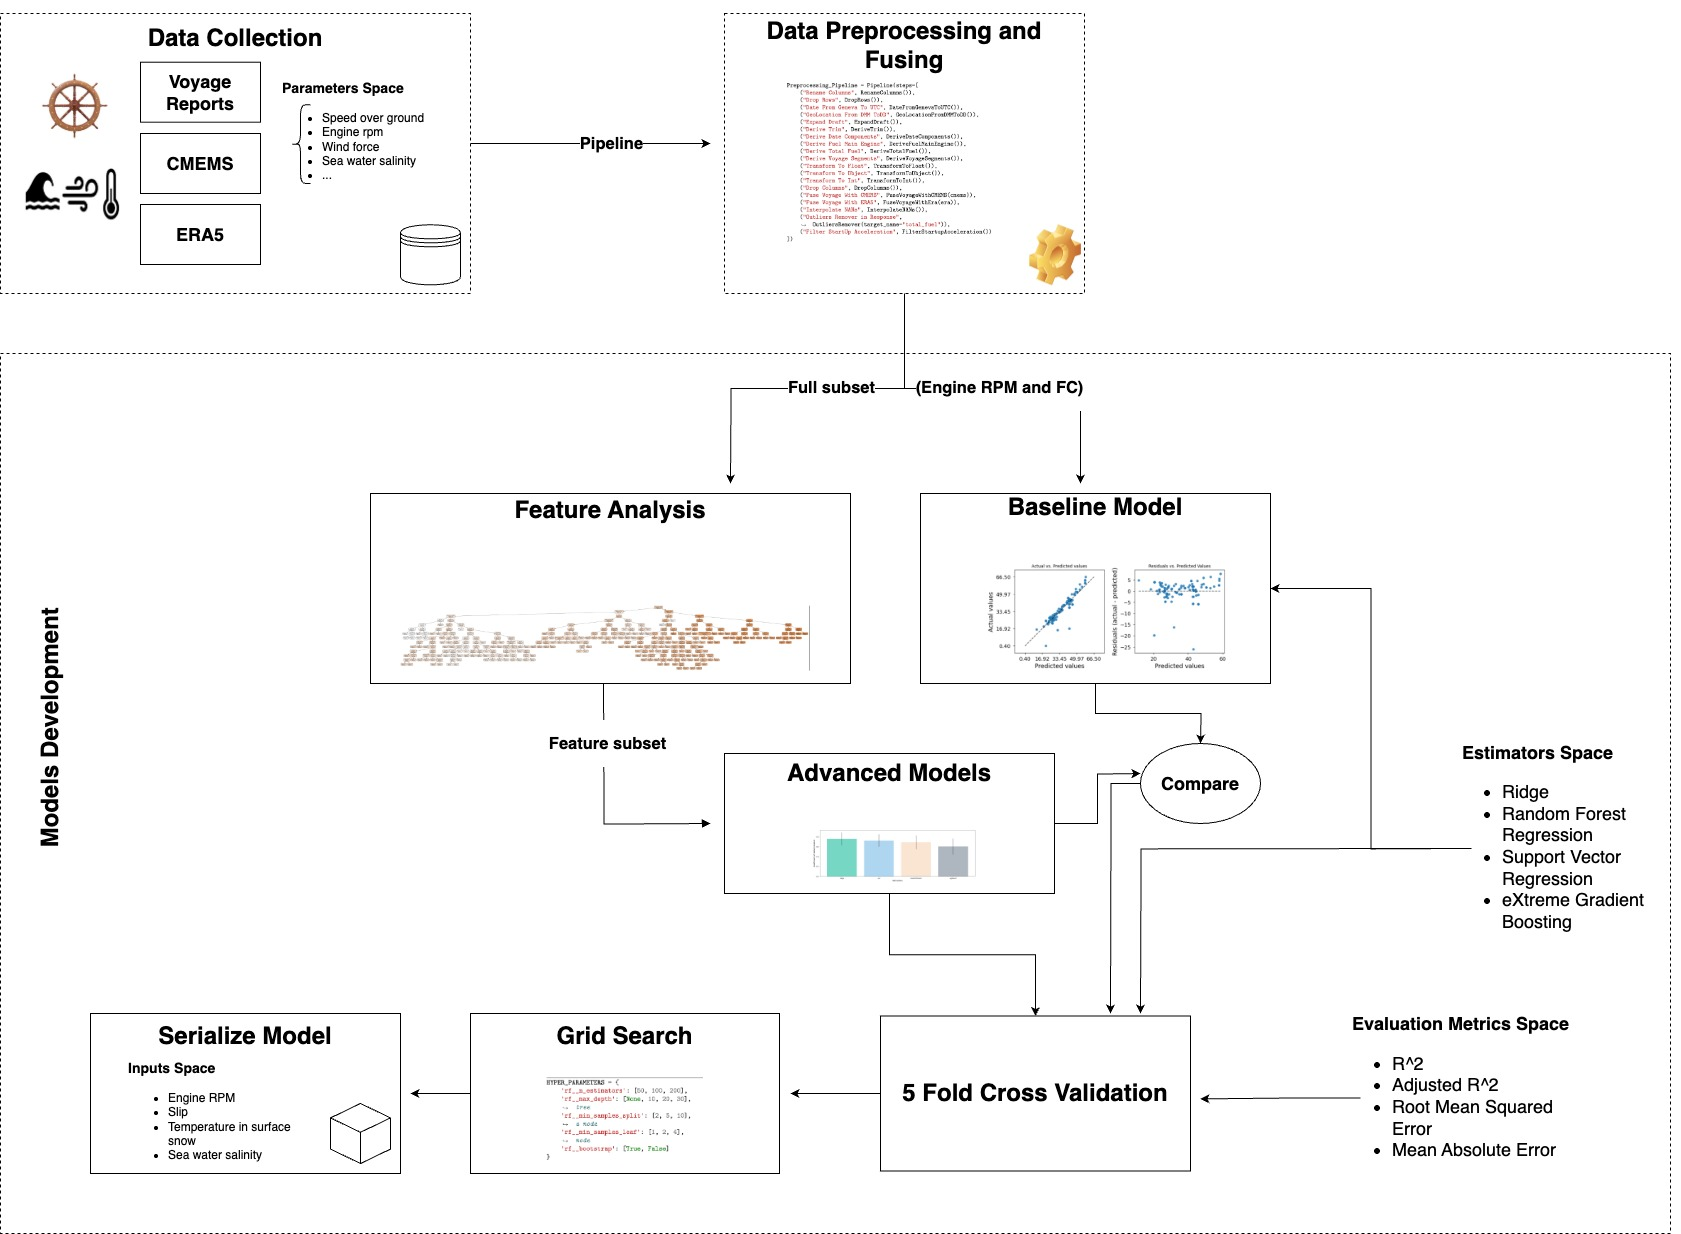
\includegraphics[width=1\linewidth]{methodological_approach}
    \caption{Illustration of Methodological Approach}
    \label{fig:methodological_approach}
\end{figure}
    
\clearpage